\documentclass{article}
\usepackage{amsrefs}
\usepackage{amssymb}
\usepackage{amsmath}
\usepackage{amsthm}
\usepackage{graphicx}

\DeclareMathOperator{\dom}{dom}
\newtheorem*{definitie}{Definitie} \newtheorem*{notatie}{Notatie} \newtheorem*{voorbeeld}{Voorbeeld}

\title{Algemene definities}
\date { }

\begin{document}

\maketitle \noindent

\noindent In de algemene definities is $y=f(x)$ het voorschrift van een functie $f$ en $a \in \dom (f)$ zodat $f$ continu is op een omgeving van $a$.
Intu\"itief betekent dit dat een open interval $I \subset \dom (f)$ bestaat dat $a$ bevat en zodat de grafiek van $f$ boven het interval $I$ geen ''sprongen'' vertoont.\vspace{5mm}

\begin{voorbeeld}
In het inleidende voorbeeld is $f(x)=1,5+50 x -4,9 x^2$, $\dom (f)= \mathbb{R}$ en $a=2$.
Deze functie is continu in 2. Je ziet hieronder de grafiek van de functie.
\begin{figure}[h]
\begin{center}
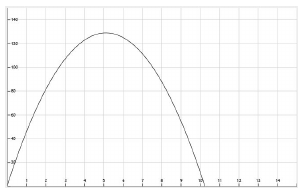
\includegraphics[height=5 cm]{graf.JPG}
\end{center}
\end{figure}
\end{voorbeeld}

Naar analogie met dit inleidende voorbeeld introduceren we de volgende definitie.

\begin{definitie}
Als de limietwaarde van $\frac{f(a+\Delta x)-f(a)}{\Delta x}$ voor $\Delta x = 0$ een re\"eel getal is dan heet dat re\"eel getal de. afgeleide van $f$ in $a$.
In dat geval zeg je dat $f$ afleidbaar is in $a$
\end{definitie}

\begin{notatie}
Als $y=f(x)$ afleidbaar is in $a$ dan zijn volgende notaties toegelaten om de afgeleide van $f$ in $a$ aan te duiden (zie Actimath cursus blz 4)
\end{notatie}

\begin{voorbeeld}
In het inleidend voorbeeld heb je voor de functie  $f(x)=1,5+50 x -4,9 x^2$ gevonden dat deze afleidbaar is in 2 en voor de afgeleide in 2 heb je gevonden dat $Df(2)=30,4$.
\end{voorbeeld}\vspace{0,5 cm}

\noindent Vanuit het inleidende voorbeeld ken je een betekenis voor de afgeleide van een functie $f$ in $a$.\vspace{0,2 cm}

\fbox{
\begin{minipage}{10 cm}
De afgeleide van $f$ in $a$ is de snelheid waarmee de functiewaarde $f(x)$ verandert als $x$ verandert vertrekkende met de waarde $x=a$
\end{minipage}}\vspace{0,5 cm}

\noindent De afgeleide heeft ook een belangrijke meetkundige betekenis.\vspace{0,2 cm}

\fbox{
\begin{minipage}{10 cm}
De afgeleide van $f$ in $a$ is de richtingsco\"effici\"ent van de raaklijn aan de grafiek van $f$ in het punt $P(a,f(a))$.
\end{minipage}}\vspace{0,2 cm}

De verklaring hiervan zie je in het filmpje na deze bladzijde.

\begin{voorbeeld}
Voor de functie $f(x)=1,5+50 x -4,9 x^2$ uit het inleidend voorbeeld berekende je dat $Df(2)=30,4$.
Het punt op de grafiek bij $x=2$ is het punt met co\"ordinaten $P(2;81,9)$.
De vergelijking van de raaklijn aan de grafiek van $f$ in $P$ is
\[
y-81,9=30,4(x-2)
\]
of nog
\[
y=30,4x+21,1
\]

\begin{figure}[h]
\begin{center}
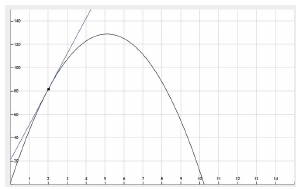
\includegraphics[height=5 cm]{grafTang.JPG}
\end{center}
\end{figure}
\end{voorbeeld}\vspace{0,5 cm}

\begin{definitie}
Als je $a$ laat vari\"eren in de punten waarin een functie $f$ afleidbaar is dan verandert $Df(a)$ (meestal) ook.
Je bekomt dan de afgeleide functie van $f$.
\end{definitie}

\begin{notatie}
Voor het aanduiden van de afgeleide functie van een functie $y=f(x)$ mag je de volgende notaties gebruiken (actimath cursus blz 7)
\end{notatie}





\end{document}